% Options for packages loaded elsewhere
\PassOptionsToPackage{unicode}{hyperref}
\PassOptionsToPackage{hyphens}{url}
\documentclass[
  spanish,
  11pt,
]{article}
\usepackage{xcolor}
\usepackage[margin=2cm]{geometry}
\usepackage{amsmath,amssymb}
\setcounter{secnumdepth}{-\maxdimen} % remove section numbering
\usepackage{iftex}
\ifPDFTeX
  \usepackage[T1]{fontenc}
  \usepackage[utf8]{inputenc}
  \usepackage{textcomp} % provide euro and other symbols
\else % if luatex or xetex
  \usepackage{unicode-math} % this also loads fontspec
  \defaultfontfeatures{Scale=MatchLowercase}
  \defaultfontfeatures[\rmfamily]{Ligatures=TeX,Scale=1}
\fi
\usepackage{lmodern}
\ifPDFTeX\else
  % xetex/luatex font selection
\fi
% Use upquote if available, for straight quotes in verbatim environments
\IfFileExists{upquote.sty}{\usepackage{upquote}}{}
\IfFileExists{microtype.sty}{% use microtype if available
  \usepackage[]{microtype}
  \UseMicrotypeSet[protrusion]{basicmath} % disable protrusion for tt fonts
}{}
\makeatletter
\@ifundefined{KOMAClassName}{% if non-KOMA class
  \IfFileExists{parskip.sty}{%
    \usepackage{parskip}
  }{% else
    \setlength{\parindent}{0pt}
    \setlength{\parskip}{6pt plus 2pt minus 1pt}}
}{% if KOMA class
  \KOMAoptions{parskip=half}}
\makeatother
\usepackage{graphicx}
\makeatletter
\newsavebox\pandoc@box
\newcommand*\pandocbounded[1]{% scales image to fit in text height/width
  \sbox\pandoc@box{#1}%
  \Gscale@div\@tempa{\textheight}{\dimexpr\ht\pandoc@box+\dp\pandoc@box\relax}%
  \Gscale@div\@tempb{\linewidth}{\wd\pandoc@box}%
  \ifdim\@tempb\p@<\@tempa\p@\let\@tempa\@tempb\fi% select the smaller of both
  \ifdim\@tempa\p@<\p@\scalebox{\@tempa}{\usebox\pandoc@box}%
  \else\usebox{\pandoc@box}%
  \fi%
}
% Set default figure placement to htbp
\def\fps@figure{htbp}
\makeatother
\ifLuaTeX
\usepackage[bidi=basic,shorthands=off]{babel}
\else
\usepackage[bidi=default,shorthands=off]{babel}
\fi
\ifLuaTeX
  \usepackage{selnolig} % disable illegal ligatures
\fi
\setlength{\emergencystretch}{3em} % prevent overfull lines
\providecommand{\tightlist}{%
  \setlength{\itemsep}{0pt}\setlength{\parskip}{0pt}}
\usepackage{titlesec}

% Remove page numbers
\pagestyle{empty}

% Section # spacing
\titlespacing*{\section}
{0pt}{1ex}{0.75ex}

% Section ## spacing
\titlespacing*{\subsection}
{0pt}{1ex}{0.5ex}

% Section ### spacing
\titlespacing*{\subsubsection}
{0pt}{0.4ex}{0.5ex}

% Paragraphs spacing
\setlength{\parskip}{0.25em}
\setlength{\parindent}{0pt}

\usepackage{enumitem}

\setlength{\parskip}{0.25em}

% Figures are floats so LaTeX decides where to place it (top, bottom, next page, etc.).
% This package force it to place it where I need
\usepackage{float}
\usepackage{placeins}
\usepackage{bookmark}
\IfFileExists{xurl.sty}{\usepackage{xurl}}{} % add URL line breaks if available
\urlstyle{same}
% fallback for those not using the hyperref driver hyperxmp:
\makeatletter
\@ifundefined{xmpquote}{\newcommand{\xmpquote}[1]{#1}}{}
\makeatother
\hypersetup{
  pdflang={es},
  hidelinks,
  pdfcreator={LaTeX via pandoc}}

\author{}
\date{}

\begin{document}

\section{1. Objetivo}\label{objetivo}

--

\section{2. Metodología}\label{metodologuxeda}

\subsection{2.1. Área de estudio}\label{uxe1rea-de-estudio}

Con el fin de estudiar el efecto de los
\href{https://www.infobae.com/salud/ciencia/2026/01/30/la-patagonia-argentina-sufre-el-incendio-mas-intenso-en-dos-decadas-segun-el-sistema-satelital-de-la-union-europea/}{incendios
ocurridos en la provincia de Chubut (Argentina) durante enero de 2026}
sobre las emisiones de \(NO_{2}\), se definió un polígono delimitado
entre \textbf{72.35°O (-72.35°) y 70.89°O (-70.89°) de longitud}, y
\textbf{43.36°S (-43.36°) y 41.95°S (-41.95°) de latitud} (ver Figura
1). De esta forma, se incluyeron las áreas del Parque Nacional Los
Alerces y las localidades de El Hoyo y Epuyén, que fueron las zonas más
afectadas por este evento.

La definición del polígono se realizó a partir del análisis realizado a
través de la plataforma
\href{https://firms.modaps.eosdis.nasa.gov/}{NASA-FIRMS}, mediante la
cual se analizó la distribución espacial de las áreas quemadas, así como
las fechas de ocurrencia de los incendios detectados por los sensores
\textbf{MODIS} y \textbf{VIIRS}.

\begin{figure}
\centering

\includegraphics[width=5.20833in,height=\textheight,keepaspectratio,alt={Mapa del área de estudio y focos de calor de MODIS registrados durante febrero de 2025 y enero de 2026.}]{report/images/fig0102.png}
\caption{Mapa del área de estudio y focos de calor de MODIS registrados
durante febrero de 2025 y enero de 2026.}
\end{figure}

\subsection{2.2. Fuentes de datos}\label{fuentes-de-datos}

\subsubsection{\texorpdfstring{2.3.1. Datos producto
\(NO_{2}\)}{2.3.1. Datos producto NO\_\{2\}}}\label{datos-producto-no_2}

Para estudiar la afectación de la calidad del aire por las emisiones de
\(NO_{2}\) producidas por los incendios ocurridos en la Patagonia
argentina, dentro del área de estudio definida (ver ítem 2.1), se
utilizó el producto \emph{offline} de nivel 2 de \(NO_{2}\) obtenido a
partir del sensor TROPOMI a bordo del satélite Sentinel-5P. Este
producto proporciona la abundancia troposférica de este contaminante en
la columna vertical, expresada en unidades de \(mol/m^{2}\).

El acceso a los datos, así como su procesamiento, se realizaron mediante
el \href{https://code.earthengine.google.com/}{editor de código de
Google Earth Engine (GEE)}. De esta forma, todas las tareas se
ejecutaron en un entorno de computación en la nube, prescindiendo del
uso de recursos computacionales locales.

Los datos de abundancia troposférica de \(NO_{2}\) se adquirieron para
dos períodos. El primero correspondió a un mes con ausencia o escasa
ocurrencia de incendios, mientras que el segundo abarcó enero de 2026,
período durante el cual se registraron los incendios objeto de este
estudio. Dentro del entorno de GEE se obtuvieron todas las escenas
disponibles para cada período y, mediante álgebra de bandas, se
generaron composiciones temporales de la cantidad de píxeles con datos
válidos (es decir, libres de nubes), así como de la suma, la mediana y
el desvío estándar de la abundancia troposférica de \(NO_{2}\) calculada
píxel a píxel.

\subsubsection{2.3.2. Datos
complementarios}\label{datos-complementarios}

Desde la plataforma NASA-FIRMS se descargaron los datos de focos de
calor detectados por el sensor MODIS correspondientes a los meses de
febrero de 2025 y enero de 2026. Estos datos proporcionan información
sobre la ocurrencia y la distribución espacial de los incendios dentro
del área de estudio. Su incorporación aporta evidencia que permite
interpretar las diferencias observadas entre los períodos seleccionados
para el análisis.

\subsection{\texorpdfstring{2.3. Análisis datos de
\(NO_{2}\)}{2.3. Análisis datos de NO\_\{2\}}}\label{anuxe1lisis-datos-de-no_2}

Los análisis implementados fueron realizado sobre las composiciones
temporales de cantidad de píxeles con datos, y la mediana y el desvío
estandar de la abundancia de \(NO_{2}\) píxel a píxel para cada periodo.
A partir de estas composiciones se llevó a cabo un primer análisis
orientado a identificar las zonas con una cantidad suficiente de datos
por píxel. Considerando que, durante el lapso de un mes, deberían
adquirirse aproximadamente 30 escenas, se estableció un umbral mínimo de
15 datos por píxel. Todos aquellos píxeles que no cumplieron con este
criterio fueron descartados.

Una vez identificadas las zonas del área de estudio que cumplían con el
umbral mínimo de datos, se continuó con el análisis de la distribución
espacial de la mediana y el desvío estándar de la abundancia de
\(NO_{2}\). Adicionalmente, se evaluó la relación entre ambos parámetros
para cada período. Esta relación se utilizó como un indicador para
determinar si la variabilidad observada en los registros de \(NO_{2}\)
respondía a una condición persistente (\(DE < \text{Mediana}\)) o a la
ocurrencia de eventos puntuales (\(DE > \text{Mediana}\)) que afectaban
la abundancia de este contaminente dentro del área de estudio.

Finalmente, se evaluaron visualmente las diferencias en la abundancia de
\(NO_{2}\) entre ambos períodos. Para ello, se emplearon gráficos
estadísticos que resumen la distribución de los datos.

\section{3. Resultados y discusión}\label{resultados-y-discusiuxf3n}

\subsection{2.1. Periodos de análisis}\label{periodos-de-anuxe1lisis}

Los períodos de análisis seleccionados fueron febrero de 2025 y enero de
2026. Esta elección se basó en el análisis de las áreas quemadas
realizado a partir de la plataforma NASA-FIRMS. Tal como se observa en
la \textbf{Figura 1}, la cantidad de focos de calor asociados a
incendios, obtenidos a partir de productos MODIS dentro del área de
estudio, fue considerablemente mayor durante enero de 2026 (1530 focos
de calor) que en febrero de 2025 (130 focos de calor). Este resultado es
consistente con los incendios de gran magnitud registrados en la región
durante 2026.

\subsection{2.2. Febrero 2025}\label{febrero-2025}

Tal como se observa en la \textbf{Figura 2}, los resultados de las
composiciones temporales para el período de febrero de 2025 muestran que
alrededor de la mitad de los píxeles se encuentran por debajo del umbral
mínimo de cantidad de datos. Estos se localizan principalmente en el
sector oeste del área de estudio, coincidiendo con la región ubicada
sobre la Cordillera de los Andes. Los datos de la mediana muestran un
rango reducido, con valores comprendidos entre -10 y 10 \(mol/m^{2}\).
Los valores negativos carecen de sentido físico y corresponden a píxeles
afectados por interferencias asociadas a la presencia de nubosidad. Por
otro lado, el desvío estándar presenta valores comprendidos entre 0 y 10
\(mol/m^{2}\).

\begin{figure}
\centering
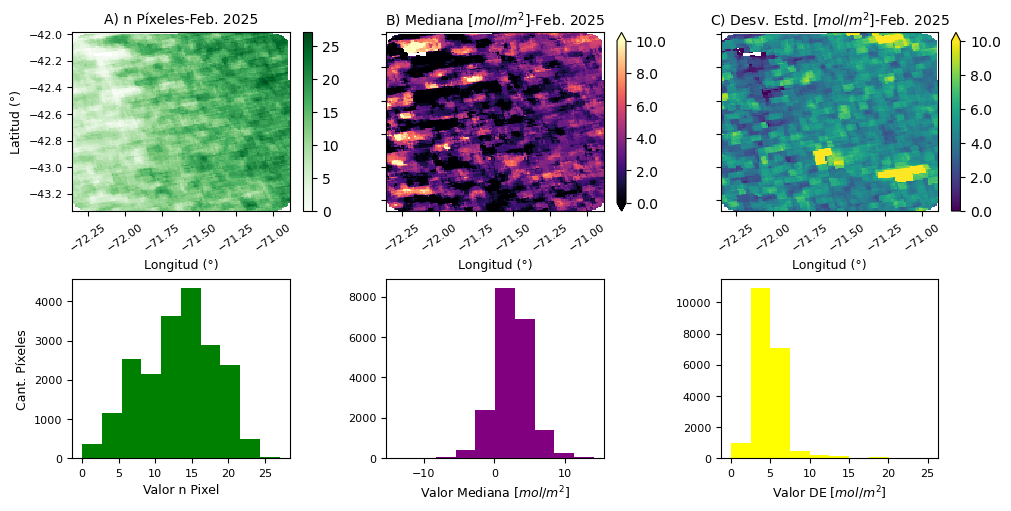
\includegraphics[width=0.8\linewidth,height=\textheight,keepaspectratio,alt={Valores computados (arriba) y distribución (abajo) de la de cantidad de píxeles válidos (A), mediana (B) y desvío estándar (C) de la abundancia de NO\_\{2\} para el área de estudio durante febrero del año 2025.}]{report/images/image0203.png}
\caption{Valores computados (arriba) y distribución (abajo) de la de
cantidad de píxeles válidos (A), mediana (B) y desvío estándar (C) de la
abundancia de \(NO_{2}\) para el área de estudio durante febrero del año
2025.}
\end{figure}

El análisis de los datos, una vez enmascarados los píxeles que no
cumplían con el umbral definido, permitió obtener un panorama más
representativo de las condiciones observadas durante el período
(\textbf{Figura 3}). Se observa un predominio de valores de mediana
entre 2 y 4 \(mol/m^{2}\), con algunas zonas que superan el valor máximo
de 10 \(mol/m^{2}\). En cuanto al desvío estándar, predominan valores
entre 4 y 6 \(mol/m^{2}\), aunque se identifican dos sectores con una
variabilidad superior a 10 \(mol/m^{2}\). Al analizar la relación entre
la mediana y el desvío estándar, se observa que en la mayor parte del
área de estudio se cumple que \(DE > \text{Mediana}\). De manera
preliminar, este resultado sugiere que durante febrero de 2025 la
abundancia de \(NO_{2}\) presentó una elevada variabilidad temporal.
Estudios posteriores podrán dilucidar si esto se debe a una cuestión
estacional o fue una situación atípica para tal época.

\begin{figure}
\centering
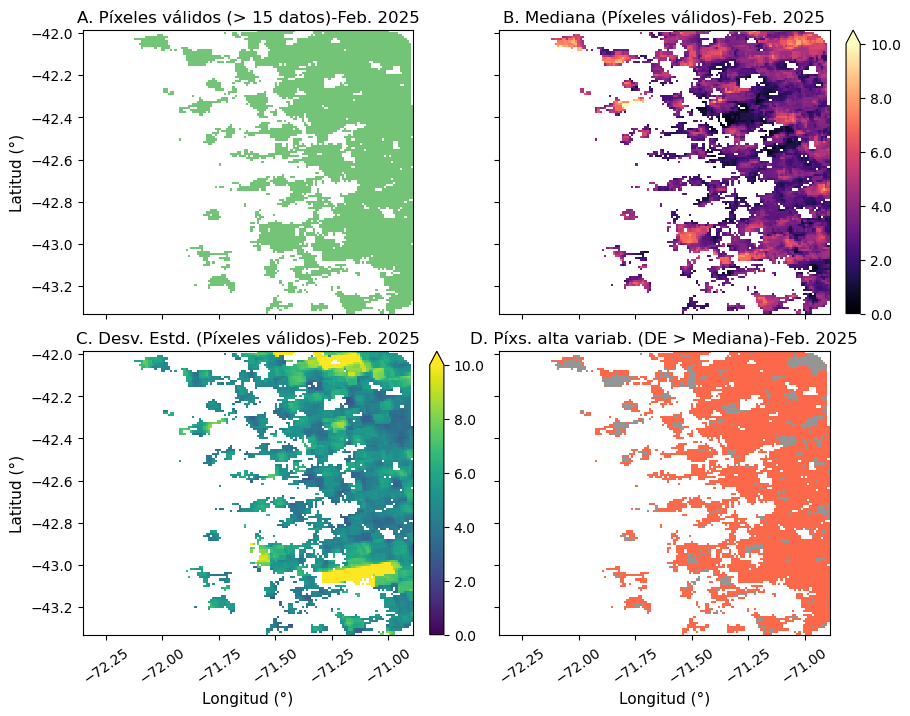
\includegraphics[width=0.7\linewidth,height=\textheight,keepaspectratio,alt={(A) Píxeles válidos dentro del área de estudio para el periodo febrero 2025. (B) Mediana computada durante febrero 2025 para los píxeles válidos dentro del área de estudio. (C) Desvío estándar computado durante febrero 2025 para los píxeles válidos dentro del área de estudio. (D) Relación entre el desvío estandar y la mediana para lo píxeles válidos. Rojo: DE \textgreater{} \textbackslash text\{Mediana\}. Gris: DE \textless{} \textbackslash text\{Mediana\}}]{report/images/image03.png}
\caption{(A) Píxeles válidos dentro del área de estudio para el periodo
febrero 2025. (B) Mediana computada durante febrero 2025 para los
píxeles válidos dentro del área de estudio. (C) Desvío estándar
computado durante febrero 2025 para los píxeles válidos dentro del área
de estudio. (D) Relación entre el desvío estandar y la mediana para lo
píxeles válidos. Rojo: \(DE > \text{Mediana}\). Gris:
\(DE < \text{Mediana}\)}
\end{figure}

\subsection{2.3. Enero 2026}\label{enero-2026}

Como se observa en la \textbf{Figura 4}, los resultados de las
composiciones temporales para el período de enero de 2026 muestran que
la mayor proporción de los píxeles se encuentra por encima del umbral
mínimo de cantidad de datos. De esta forma, la mayor parte de la
composición generada resulta apta para los análisis posteriores. Los
valores de la mediana muestran una mayor dispersión y un corrimiento
hacia valores más altos, observándose un rango comprendido entre -5 y 10
\(mol/m^{2}\), con máximos cercanos a los 20 \(mol/m^{2}\). Al igual que
en el caso anterior, los valores negativos carecen de sentido físico y
corresponden a píxeles afectados por interferencias asociadas a la
presencia de nubes. Por otro lado, el desvío estándar presenta valores
comprendidos entre 0 y 20 \(mol/m^{2}\), registrándose máximos cercanos
a los 200 \(mol/m^{2}\).

\begin{figure}
\centering
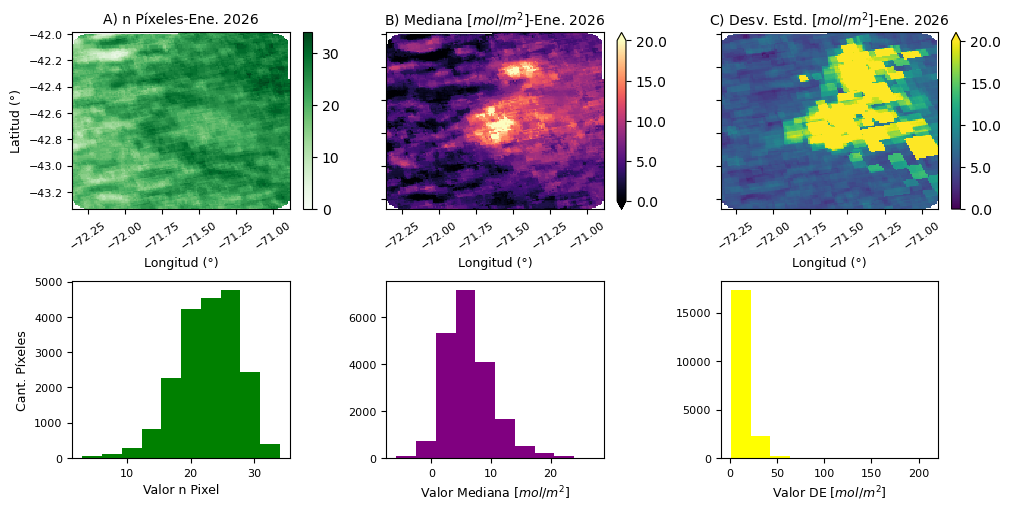
\includegraphics[width=0.8\linewidth,height=\textheight,keepaspectratio,alt={Valores computados (arriba) y distribución (abajo) de la de cantidad de píxeles válidos (A), mediana (B) y desvío estándar (C) de la abundancia de NO\_\{2\} para el área de estudio durante enero del año 2026.}]{report/images/image04.png}
\caption{Valores computados (arriba) y distribución (abajo) de la de
cantidad de píxeles válidos (A), mediana (B) y desvío estándar (C) de la
abundancia de \(NO_{2}\) para el área de estudio durante enero del año
2026.}
\end{figure}

Una vez enmascarados los píxeles que no cumplían con el umbral
establecido, su análisis (\textbf{Figura 5}) mostró un predominio de
valores de mediana entre 5 y 10 \(mol/m^{2}\), así como la presencia de
dos grandes núcleos con abundancias superiores a 15 \(mol/m^{2}\). Por
su ubicación, que puede verificarse en la \textbf{Figura 1}, estos
núcleos se asocian al incremento de \(NO_{2}\) producido por la quema de
biomasa durante los incendios ocurridos en ese período. En cuanto al
desvío estándar, predominan valores entre 5 y 10 \(mol/m^{2}\), aunque
también se observan extensas áreas con valores superiores a 20
\(mol/m^{2}\), de igual forma asociadas por su localización a los
incendios registrados. Al analizar la relación entre la mediana y el
desvío estándar, se observa que en la mayor parte del área de estudio se
cumple que \(DE > \text{Mediana}\). En conjunto, estos resultados
indican una elevada variabilidad temporal en la abundancia de
\(NO_{2}\), consistente con el impacto de los incendios sobre la calidad
del aire debido al incremento de las emisiones de este contaminante.

\begin{figure}
\centering
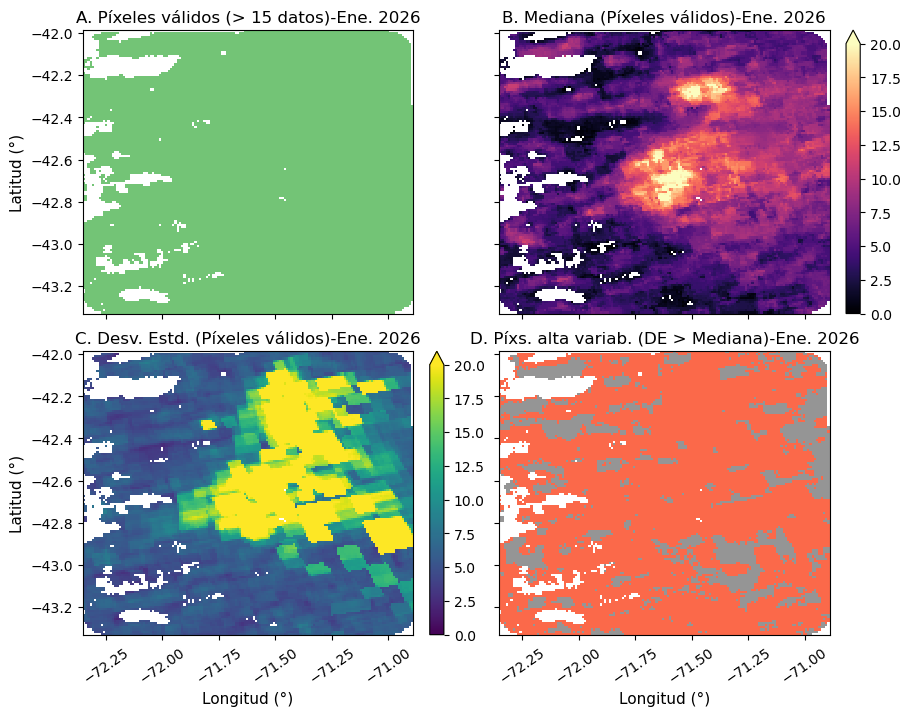
\includegraphics[width=0.7\linewidth,height=\textheight,keepaspectratio,alt={(A) Píxeles válidos dentro del área de estudio para el periodo enero 2026. (B) Mediana computada durante enero 2026 para los píxeles válidos dentro del área de estudio. (C) Desvío estándar computado durante enero 2026 para los píxeles válidos dentro del área de estudio. (D) Relación entre el desvío estandar y la mediana para lo píxeles válidos. Rojo: DE \textgreater{} \textbackslash text\{Mediana\}. Gris: DE \textless{} \textbackslash text\{Mediana\}}]{report/images/image05.png}
\caption{(A) Píxeles válidos dentro del área de estudio para el periodo
enero 2026. (B) Mediana computada durante enero 2026 para los píxeles
válidos dentro del área de estudio. (C) Desvío estándar computado
durante enero 2026 para los píxeles válidos dentro del área de estudio.
(D) Relación entre el desvío estandar y la mediana para lo píxeles
válidos. Rojo: \(DE > \text{Mediana}\). Gris: \(DE < \text{Mediana}\)}
\end{figure}

\subsection{2.4. Comparación entre
periodos}\label{comparaciuxf3n-entre-periodos}

La comparación de la mediana de la abundancia de \(NO_{2}\) entre ambos
períodos mediante el gráfico de caja (\emph{boxplot}) de la
\textbf{Figura 6} muestra una diferencia marcada en la tendencia central
de los datos dentro del área de estudio. En particular, la mediana
aproximadamente se duplicó durante los incendios de enero de 2026.
Asimismo, el rango intercuartílico es mayor en este período, lo que
indica una mayor heterogeneidad espacial en la abundancia de \(NO_{2}\).
Finalmente, la presencia de numerosos valores\emph{outliers} evidencia
la existencia de zonas con abundancias excepcionalmente elevadas de
\(NO_{2}\), las cuales podrían estar asociadas directamente a las
emisiones producidas por los focos de incendio.

\end{document}
